\documentclass[11pt]{amsart}
\usepackage{amssymb,amsmath,latexsym,times,enumitem,tikz,soul}

\setstcolor{red}
\setul{0pt}{1.5pt}

\addtolength{\evensidemargin}{-40pt}
\addtolength{\oddsidemargin}{-40pt}
\addtolength{\textwidth}{80pt}
\addtolength{\textheight}{80pt}
\addtolength{\topmargin}{-40pt}

\pagestyle{empty}

\begin{document}

\noindent
{\textbf{\color{blue}Charlene R. Ramos}}\\
ECON 280 Computation Fall 2024\\
Part \# 2: Choosing Your Project to Replicate\\
Wednesday, October 23, 2024\\

\smallskip 

\noindent Bloom, Nicholas, Charles I. Jones, John Van Reenen, and Michael Webb. ``Are Ideas Getting Harder to Find?'' \emph{American Economic Review} 2020, 110 (4): 1104–1144.\\ 

\noindent {\textbf{\color{blue}Research Question \& Contribution}}

\smallskip

\noindent Bloom et al. (2020) posits a production function for new ideas described by the equation: 

\begin{center}
\emph{economic growth = research productivity x number of researchers.}
\end{center}

\noindent Such a model is representative of macroeconomic research studying long-run growth due to innovation. The authors leverage microeconomic datasets on firms including Compustat and Census Bureau to demonstrate that research effort has increased significantly while research productivity has decreased substantially. Their case studies span from agricultural yields to semiconductors in manufacturing as well as medical technologies like new molecular entities to emphasize that this trend appears across a wide range of disparate industries. The authors frame their research contributions as the following: 1) to examine multiple layers of aggregate evidence at once; 2) to derive a conceptually consistent approach from core growth models that align with these layers; and, 3) to provide additional context for the kind of models found in growth literature. 

\bigskip

\bigskip

\noindent {\textbf{\color{blue}Empirical Framework}}

\smallskip

\noindent Bloom et al. (2020) contextualizes the canonical Solow growth model to empirically evaluate the idea production model at the micro level. The authors choose research and development (R \& D) expenditures rather than number of researchers to calculate research productivity. They deflate R \& D spending by the economy's wage rate using the mean personal income from the Current Population Survey for males with a bachelor's degree education. From there, the authors create a measure of the number of researchers that R \& D spending could purchase. They interpret the measure as the number of ``effective scientists'' and also refer to it as ``research effort.''  

\bigskip

\bigskip

\noindent {\textbf{\color{blue}Structure of Dataset}}

\smallskip

\noindent Prior to running ``MasterIdeaPF.m'', the master program for all results other than Census, the Compustat data must get cleaned in ``CompustatRead.m.'' ``CompustatRead.m'' brings in ``CompustatRawData.mat'' to include only relevant data; for instance, the script drops missing or duplicate observations and keeps data from $1980$ onwards. From there, ``CompustatData\_.mat'' is saved as $35$ variables that span $36$ years and represent $15,128$ firms. Some of the variables like sales revenue or market capitalization are measured in dollars (both as real and nominal). There also exist dummy variables per decade such as $1980$s, $1990$s, $2000$s, and $2010$s to compare among firms across time. 

\newpage

\noindent {\textbf{\color{blue}Histogram}}

\smallskip

\noindent The histogram plots the interquartile range of research and development expenditures in million dollars by $2,131$ firms during the year $2015$. 

\begin{figure}[h]
    \centering 
    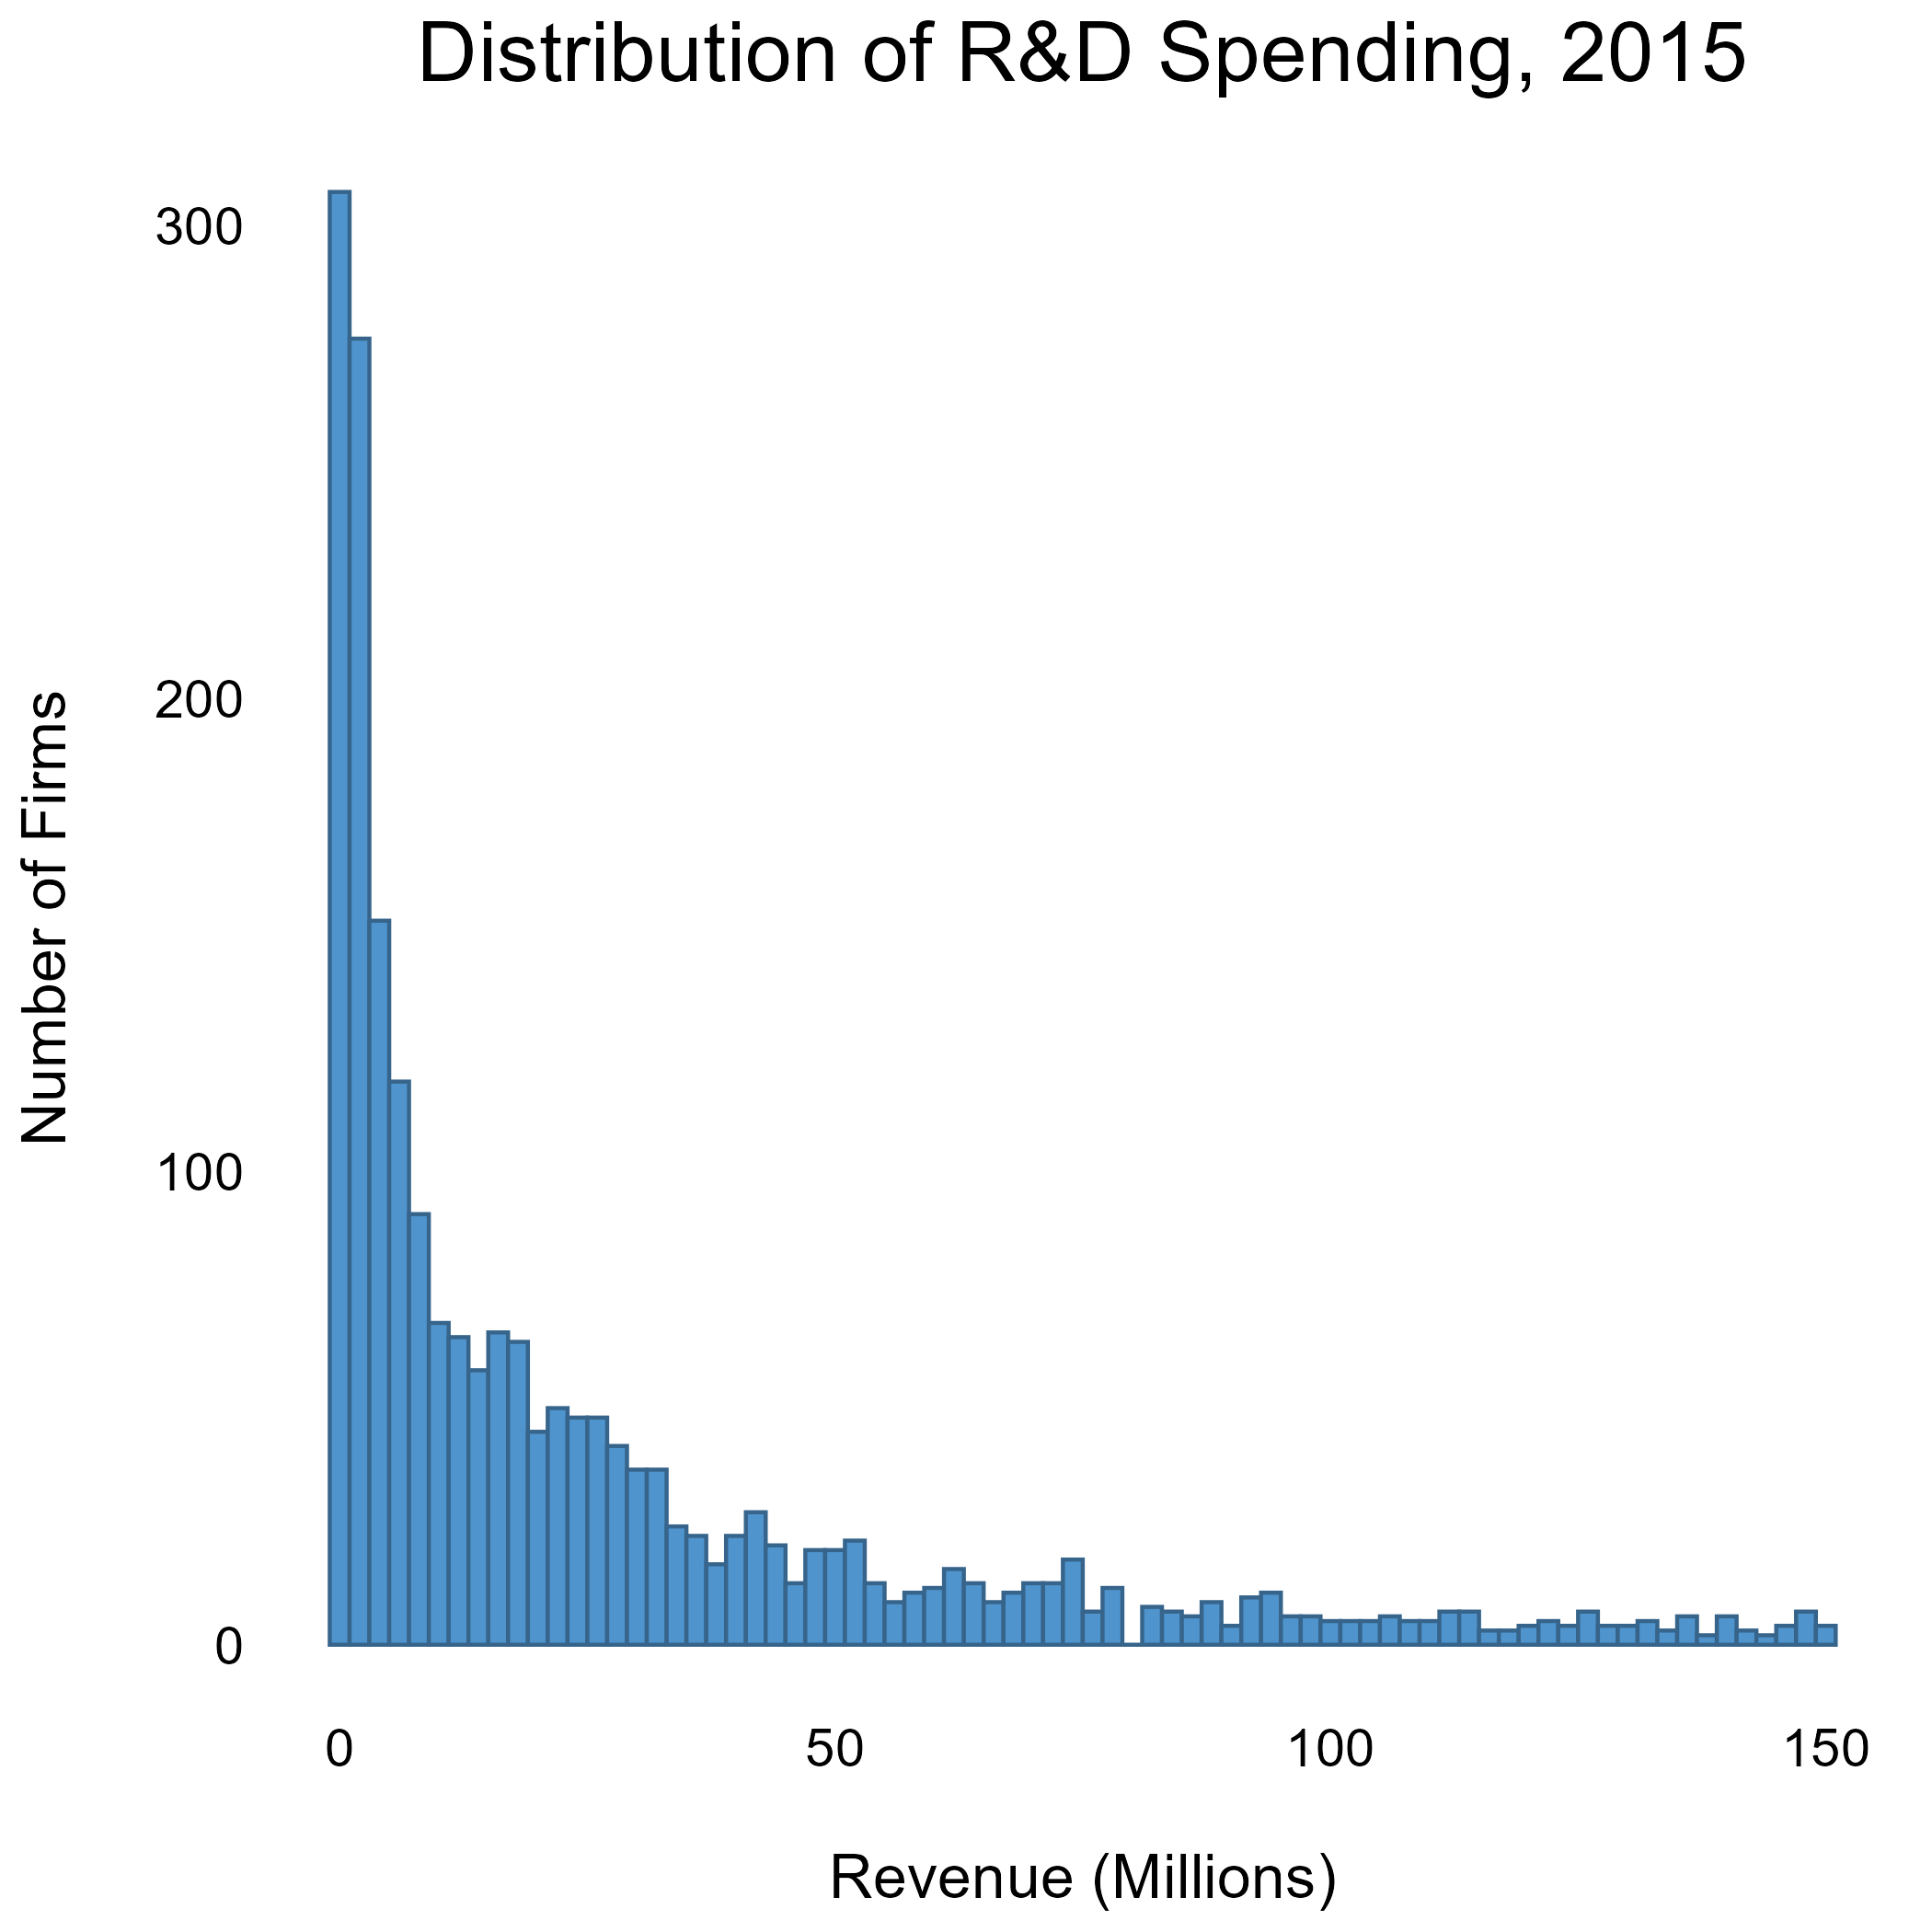
\includegraphics[width=0.8\textwidth]{histogram.png}  
    \label{fig:histogram} 
\end{figure}

\noindent

\end{document}

